\documentclass{beamer}

\usepackage[utf8]{inputenc}

\usetheme{Madrid}
\usecolortheme{seahorse}
\usefonttheme{structuresmallcapsserif}
\setbeamercovered{dynamic}

\title{Exposée Sensorik}
\author[Y. Höll, G. Muck, C. Pooch, G. N. Tchapda]
	{Yannik~Höll \\ \and Georg~Muck \\ \and Christoph~Pooch \\ \and  Gwladys Noutep Tchapda}
\date{22.04.2021}
\logo{
\includegraphics[]{TUBAF-logo.png}}

\beamertemplatenavigationsymbolsempty 

\begin{document}
	\frame{\titlepage}

\AtBeginSection[]{
  \begin{frame}
  \vfill
  \centering
  \begin{beamercolorbox}[sep=8pt,center,shadow=true,rounded=true]{title}
    \usebeamerfont{title}\insertsectionhead\par%
  \end{beamercolorbox}
  \vfill
  \end{frame}
}

\begin{frame}
\frametitle{Einteilung}
\tableofcontents
\end{frame}

\section{Motivation}
\begin{frame}
\frametitle{Motivation}
\begin{itemize}
\item<1-> Ziel: Roboter der sinnvoll über Campus fahren soll
\begin{itemize}
\item<2-4> sinnvolle Navigation
\item<3-4> beachten von Hindernissen wie Menschen oder Schlaglöchern
\item<4> ggf erkennen von Fehlern in anderen Bereichen
\end{itemize}

\item<5-> akkurate \alert<6->{Aufnahme}, \alert<6->{Verarbeitung} und (durch \alert<6->{Verarbeitung}) sinnvolle \alert<6->{Bereitstellung} der Sensordaten
\end{itemize}
\end{frame}


\section{Organisation \& Ablauf}
\begin{frame}
\frametitle{Organisation \& Ablauf}
\begin{itemize}
\item<1-> \alert{Meeting} am Anfang und am Ende der "Arbeitswoche"
\item<2-> Aufgaben zu geregelten Zeiten erledigen
\item<3-> feste \alert{Verbindlichkeiten}
\item<4-> Kommunikation via \alert{Discord} und Datenaustausch via \alert{GitHub}
\end{itemize}
\end{frame}

\begin{frame}
\frametitle{Organisation \& Ablauf - Wochen 1 bis 6}
\begin{itemize}
\item<1-> Vorbereitung (Woche 1 - 2)
\begin{itemize}
\item<2-6> Definieren des Problems
\item<3-6> Recherche Sensoren
\item<4-6> Sichten Bibliotheken
\item<5-6> Erstellen UML-Klassendiagramme
\item<6> Festlegung Zugriffsverfahren
\end{itemize}
\item<7-> Recherche \& Planung (Woche 3 - 6)
\begin{itemize}
\item<8-11> Grobe Implementierung Sensoren
\item<9-11> Testen Bibliotheken
\item<10-11> Testen Sensoren
\item<11> Implementierung Datenformate in ROS
\end{itemize}
\end{itemize}
\end{frame}

\begin{frame}
\frametitle{Organisation \& Ablauf - Wochen 7 bis 14}
\begin{itemize}
\item<1-> Verfeinerung (Woche 7 - 11)
\begin{itemize}
\item<2-3> Implementierung Filterungsalgorithmen
\item<3> Verarbeitung der Daten in das vereinbarte Format
\end{itemize}
\item<4-> Integration (Woche 12 - 14)
\begin{itemize}
\item<5-6> Integration in Husky
\item<6> gegebenenfalls Bugs beheben
\end{itemize}
\end{itemize}
\end{frame}

\section{Stand der Technik}
\begin{frame}
\frametitle{Stand der Technik - Odometrie}
\begin{itemize}
\item<1> bereits nativ im System integriert
\end{itemize}
\end{frame}

\begin{frame}
\frametitle{Stand der Technik - LiDAR Sensor}
	\begin{figure}[h!]
  		\caption{Auszug Datenblatt LiDAR TiM551}
		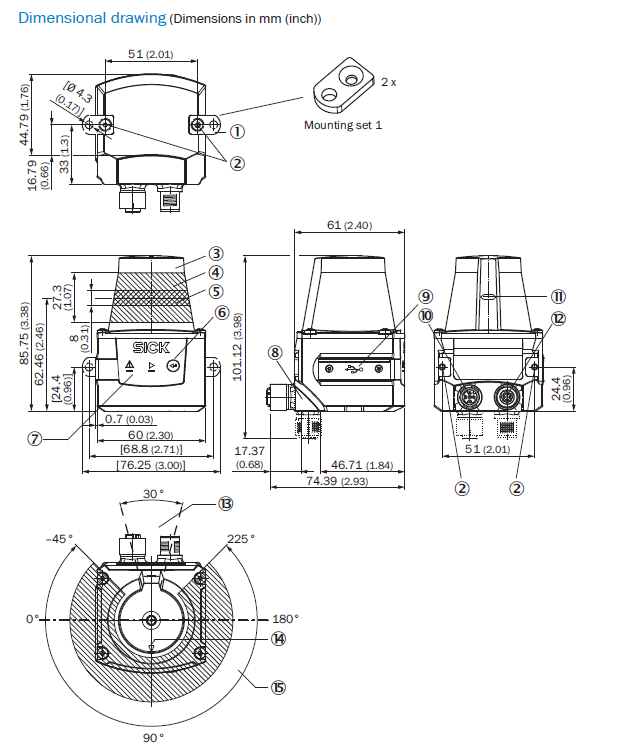
\includegraphics[width = 170px, height = 170px]{LidarTim551Drawing.PNG}	
	\end{figure}
\end{frame}

\begin{frame}
\frametitle{Stand der Technik - LiDAR Sensor}
\begin{itemize}
\item<1-> Reichweite: 10m 
\item<2-> misst zwischen -45° und 225°
\item<3-> sendet Distanz in Gradintervallen
\item<4> drei Echos
\end{itemize}
\end{frame}

\begin{frame}
\frametitle{Stand der Technik - Ausgabebeispiel}
	\begin{figure}[h!]
  		\caption{Ausgabebeispiel LiDAR TiM551}
		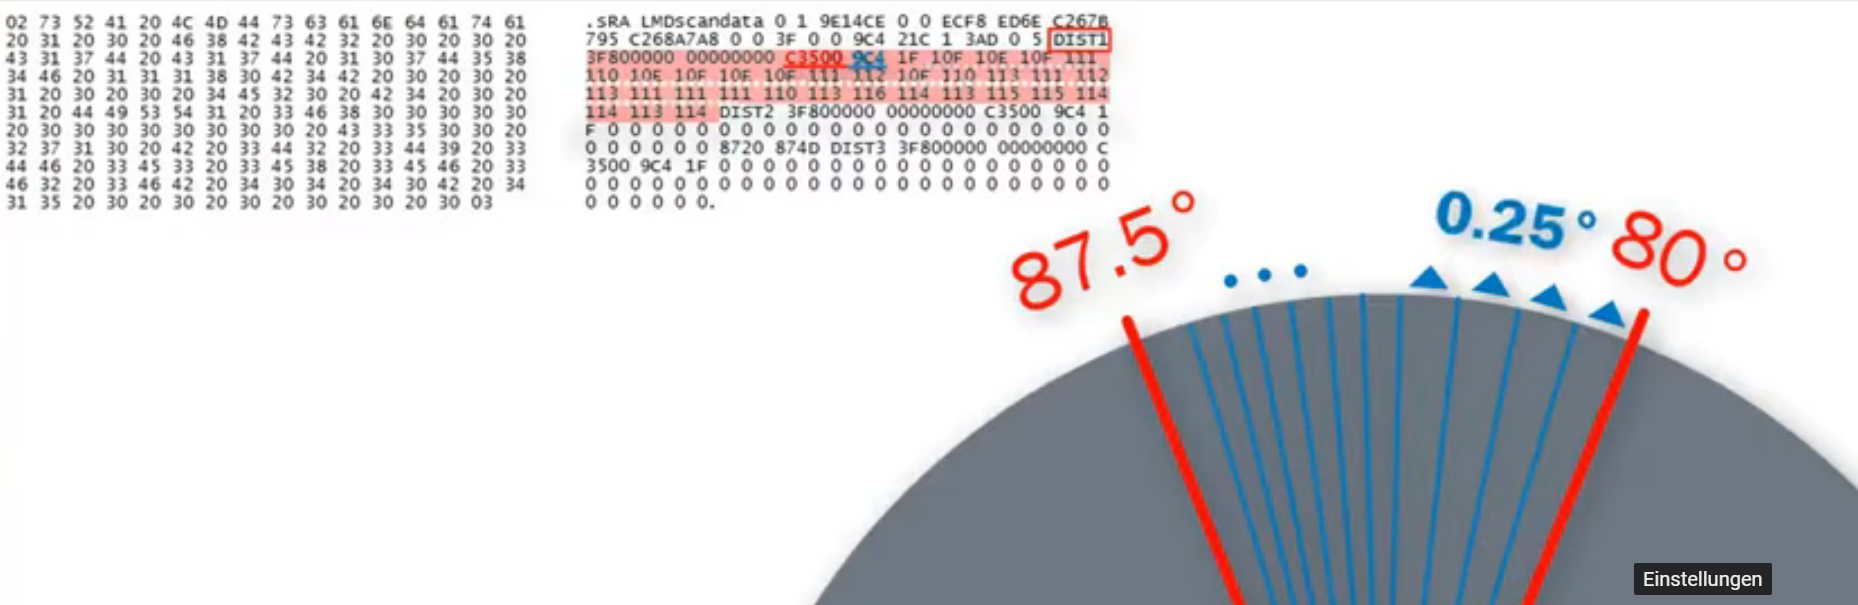
\includegraphics[width = 330px, height = 170px]{Lidar-OutputExample.PNG}	
	\end{figure}
\end{frame}

\begin{frame}
\frametitle{Stand der Technik - GNSS}
\begin{itemize}
\item<1-> arbeitet mit Galileo-Satelliten
\item<2-> bis zu 72 Satelliten gleichzeitig
\item<3-> Treiber für Linux und Windows verfügbar
\item<4> Unterstützt C\#/C++/VB
\end{itemize}
\end{frame}

\begin{frame}
\frametitle{Stand der Technik - GNSS}
	\begin{figure}[h!]
  		\caption{uBlox8 Produktbild}
		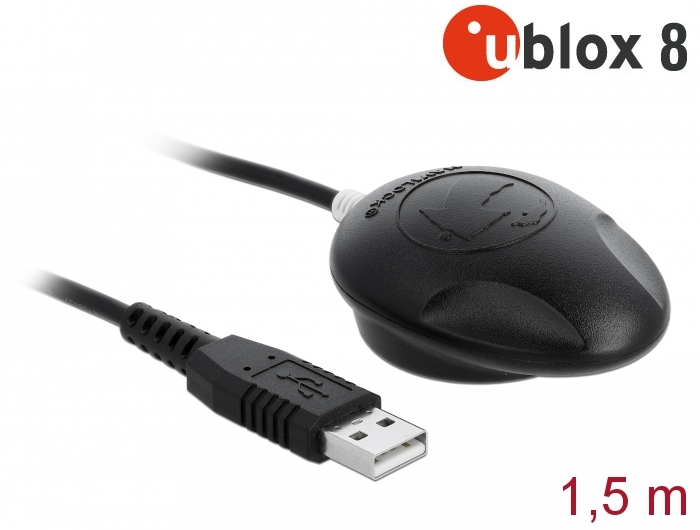
\includegraphics[width = 230px, height = 170px]{uBlox8.jpg}	
	\end{figure}
\end{frame}

\end{document}
